\documentclass{standalone}
\usepackage{fontspec}
\setmainfont{Arial}
\usepackage{tikz}
\usepackage{xcolor}
\usetikzlibrary{arrows.meta, positioning, shapes.geometric, 3d, calc}
\usepackage{tikz-3dplot}
\tikzset{plane/.style n args={3}{insert path={%
#1 -- ++ #2 -- ++ #3 -- ++ ($-1*#2$) -- cycle}},
unit xy plane/.style={plane={#1}{(1,0,0)}{(0,1,0)}},
unit xz plane/.style={plane={#1}{(1,0,0)}{(0,0,1)}},
unit yz plane/.style={plane={#1}{(0,1,0)}{(0,0,1)}},
get projections/.style={insert path={%
let \p1=(1,0,0),\p2=(0,1,0)  in 
[/utils/exec={\pgfmathtruncatemacro{\xproj}{sign(\x1)}\xdef\xproj{\xproj}
\pgfmathtruncatemacro{\yproj}{sign(\x2)}\xdef\yproj{\yproj}
\pgfmathtruncatemacro{\zproj}{sign(cos(\tdplotmaintheta))}\xdef\zproj{\zproj}}]}},
pics/unit cube/.style={code={
\path[get projections];
\draw (0,0,0) -- (1,1,1);
\ifnum\zproj=-1
 \path[3d cube/every face,3d cube/xy face,unit xy plane={(0,0,0)}]; 
\fi
\ifnum\yproj=1
 \path[3d cube/every face,3d cube/yz face,unit yz plane={(1,0,0)}]; 
\else
 \path[3d cube/every face,3d cube/yz face,unit yz plane={(0,0,0)}]; 
\fi
\ifnum\xproj=1
 \path[3d cube/every face,3d cube/xz face,unit xz plane={(0,0,0)}]; 
\else
 \path[3d cube/every face,3d cube/xz face,unit xz plane={(0,1,0)}]; 
\fi
\ifnum\zproj>-1
 \path[3d cube/every face,3d cube/xy face,unit xy plane={(0,0,1)}]; 
\fi
}},
3d cube/.cd,
xy face/.style={fill=blue!10},
xz face/.style={fill=blue!20},
yz face/.style={fill=blue!30},
num cubes x/.estore in=\NumCubesX,
num cubes y/.estore in=\NumCubesY,
num cubes z/.estore in=\NumCubesZ,
num cubes x=1,num cubes y/.initial=1,num cubes z/.initial=1,
cube scale/.initial=0.9,
every face/.style={draw,very thick},
/tikz/pics/.cd,
cube array/.style={code={%
 \tikzset{3d cube/.cd,#1}
 %\typeout{\NumCubesX,\NumCubesY,\NumCubesZ}
  \path[get projections];
  \ifnum\yproj=1
   \def\LstX{1,...,\NumCubesX}
  \else 
   \ifnum\NumCubesX>1
    \pgfmathtruncatemacro{\NextToLast}{\NumCubesX-1}
    \def\LstX{\NumCubesX,\NextToLast,...,1}
   \else
    \def\LstX{1}   
   \fi 
  \fi
  \ifnum\xproj=-1
   \def\LstY{1,...,\NumCubesY}
  \else 
   \ifnum\NumCubesY>1
    \pgfmathtruncatemacro{\NextToLast}{\NumCubesX-1}
    \def\LstY{\NumCubesY,\NextToLast,...,1}
   \else
    \def\LstY{1}   
   \fi 
  \fi
  \ifnum\zproj=1
   \def\LstZ{1,...,\NumCubesZ}
  \else 
   \ifnum\NumCubesZ>1
    \pgfmathtruncatemacro{\NextToLast}{\NumCubesX-1}
    \def\LstZ{\NumCubesZ,\NextToLast,...,1}
   \else
    \def\LstZ{1}   
   \fi 
   \def\LstZ{\NumCubesZ,\NextToLast,...,1}
  \fi
  \foreach \X in \LstX
  {\foreach \Y in \LstY
   {\foreach \Z in \LstZ
    {
    \ifnum\X=4
      \ifnum\Y=2
        \path (\X-\NumCubesX/2-1,\Y-\NumCubesY/2-1,\Z-\NumCubesZ/2-1)
          pic[scale=\pgfkeysvalueof{/tikz/3d cube/cube scale},
               3d cube/.cd,
               xy face/.style={fill=red!10},
               xz face/.style={fill=red!20},
               yz face/.style={fill=red!30}]{unit cube};
      \else
        \path (\X-\NumCubesX/2-1,\Y-\NumCubesY/2-1,\Z-\NumCubesZ/2-1)
          pic[scale=\pgfkeysvalueof{/tikz/3d cube/cube scale}]{unit cube};
      \fi
    \else
      \path (\X-\NumCubesX/2-1,\Y-\NumCubesY/2-1,\Z-\NumCubesZ/2-1)
        pic[scale=\pgfkeysvalueof{/tikz/3d cube/cube scale}]{unit cube};
    \fi
  }}
  } 
}}
}

\definecolor{blueBase}{RGB}{70,130,180}
\definecolor{blueLeaf}{RGB}{135,206,250}

\definecolor{greenBase}{RGB}{34,139,34}
\definecolor{greenLeaf}{RGB}{144,238,144}

\definecolor{orangeBase}{RGB}{255,140,0}
\definecolor{orangeLeaf}{RGB}{255,200,120}

\definecolor{purpleBase}{RGB}{138,43,226}
\definecolor{purpleLeaf}{RGB}{186,85,211}

\definecolor{redBase}{RGB}{178,34,34}
\definecolor{redLeaf}{RGB}{240,128,128}

\definecolor{grayBase}{RGB}{105,105,105}
\definecolor{grayLeaf}{RGB}{169,169,169}

\definecolor{lightblue}{RGB}{225,245,254}
\definecolor{highlightblue}{RGB}{144,202,249}

\definecolor{lightgray}{RGB}{240,240,240}
\definecolor{highlightgray}{RGB}{200,200,200}

\definecolor{darkgreenMW}{RGB}{0, 170, 0} % or choose your own color
\definecolor{lightgreenMW}{RGB}{144,238,144}
\definecolor{darkgreenMW}{RGB}{0, 170, 0} % or choose your own color
\definecolor{lightgreenMW}{RGB}{144,238,144}

\begin{document}

    \tdplotsetmaincoords{60}{45} 
    % the first argument cannot be larger than 90
    \begin{tikzpicture}[tdplot_main_coords, line join=round, 3d cube/.cd,
        num cubes x=4, num cubes y=4, num cubes z=4]
        \node[font=\large] at (-8,1) {(A)};
        \path pic {cube array={}};

        Longitude, Latitude, Time) aligned with cube edges
        % Make sure you're inside this scope:
        \begin{scope}[tdplot_main_coords]
            
            % Arrow: Longitude (X-axis): from left-bottom-front to middle-bottom-front
            \draw[->, thick, orangeBase]
            (-2.5, -2.5, -2.5) -- (3, -3, -2)
            node[midway, below, sloped] {Longitude};
            
            % Arrow: Latitude (Y-axis): from middle-bottom-front to right-bottom-front
            \draw[->, thick, grayLeaf]
            (3, -3, -2) -- (3, 2, -2)
            node[midway, below, sloped] {Latitude};
            % Arrow: Time (Z-axis): from bottom-left to top-left
            \draw[->, thick, greenBase]
            (-2.5, -2.5, -2.5) -- (-2, -3, 2)
            node[midway, left] {\shortstack{Time\\(Years)}};

            \draw[->, thick, red!70]
            (2,-1.2, 2.4)..controls(0,0.5,2.2)..(0.7,0.7,3.5);
            
            \node[text=black] at (1,1,3.9) {Time series bin};

        \end{scope}
        
    \end{tikzpicture}

        \centering
        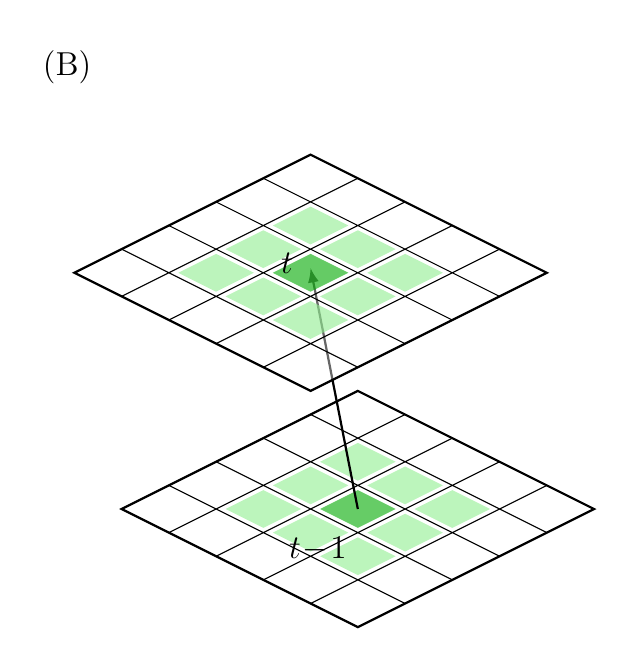
\begin{tikzpicture}[scale=.6, every node/.style={minimum size=1cm}]
        \node[anchor=north west, font=\large] at (-6,7.7) {(B)};
        % Define grid and insets
        \def\gridsize{5}
        \def\cellsize{1}
        \def\inset{0.1} % amount to inset the fill from each side
        
        % Function to draw filled cell with inset
        \newcommand{\fillcell}[3]{
            \fill[#3, fill opacity = 0.6] (#1+\inset,#2+\inset) rectangle (#1+1-\inset,#2+1-\inset);
            }
            
        % === First Grid (lower, 3D perspective) ===
        \begin{scope}[yshift=-5cm, xshift=1cm, every node/.append style={yslant=0.5,xslant=-1}, yslant=0.5, xslant=-1]
            \draw[step=\cellsize, black] (0,0) grid (\gridsize,\gridsize);
            \draw[black, thick] (0,0) rectangle (\gridsize,\gridsize);

  % Center cell
  \fillcell{2}{2}{darkgreenMW}

  % 8-neighbourhood
  \foreach \x/\y in {1/1, 1/2, 1/3, 2/1, 2/3, 3/1, 3/2, 3/3} {\fillcell{\x}{\y}{lightgreenMW}}
\end{scope}

% === Arrow (behind top grid) ===
\coordinate (center_tminus1) at (1,3.5-6); % center of bottom grid
\coordinate (center_t) at (0,2.6);       % center of top grid
\draw[-latex, thick, black] (center_tminus1) -- (center_t);
\node[below left, font=\bfseries\large] at (center_tminus1) {$t\!-\!1$};

% === Second Grid (upper, semi-transparent overlay) ===
\begin{scope}[yshift=0cm, every node/.append style={yslant=0.5,xslant=-1}, yslant=0.5, xslant=-1]
  \fill[white, fill opacity=0.4] (0,0) rectangle (\gridsize,\gridsize);
  \draw[step=\cellsize, black] (0,0) grid (\gridsize,\gridsize);
  \draw[black, thick] (0,0) rectangle (\gridsize,\gridsize);

  % Center cell
  \fillcell{2}{2}{darkgreenMW}

  % 8-neighbourhood
  \foreach \x/\y in {1/1, 1/2, 1/3, 2/1, 2/3, 3/1, 3/2, 3/3} {\fillcell{\x}{\y}{lightgreenMW}}
\end{scope}

% === Annotations ===
\node[font=\bfseries\large] at (-0.5,2.7) {$t$}; % Position manually above the top grid

        \end{tikzpicture}

\end{document}